\newpage 

\section{Sharding Data \& Consistent Hashing}
\label{sec:shard}

Say we have a 1 TB dataset with only 5 servers each with 200 GB of storage.

\begin{figure}[h]

    \centering
    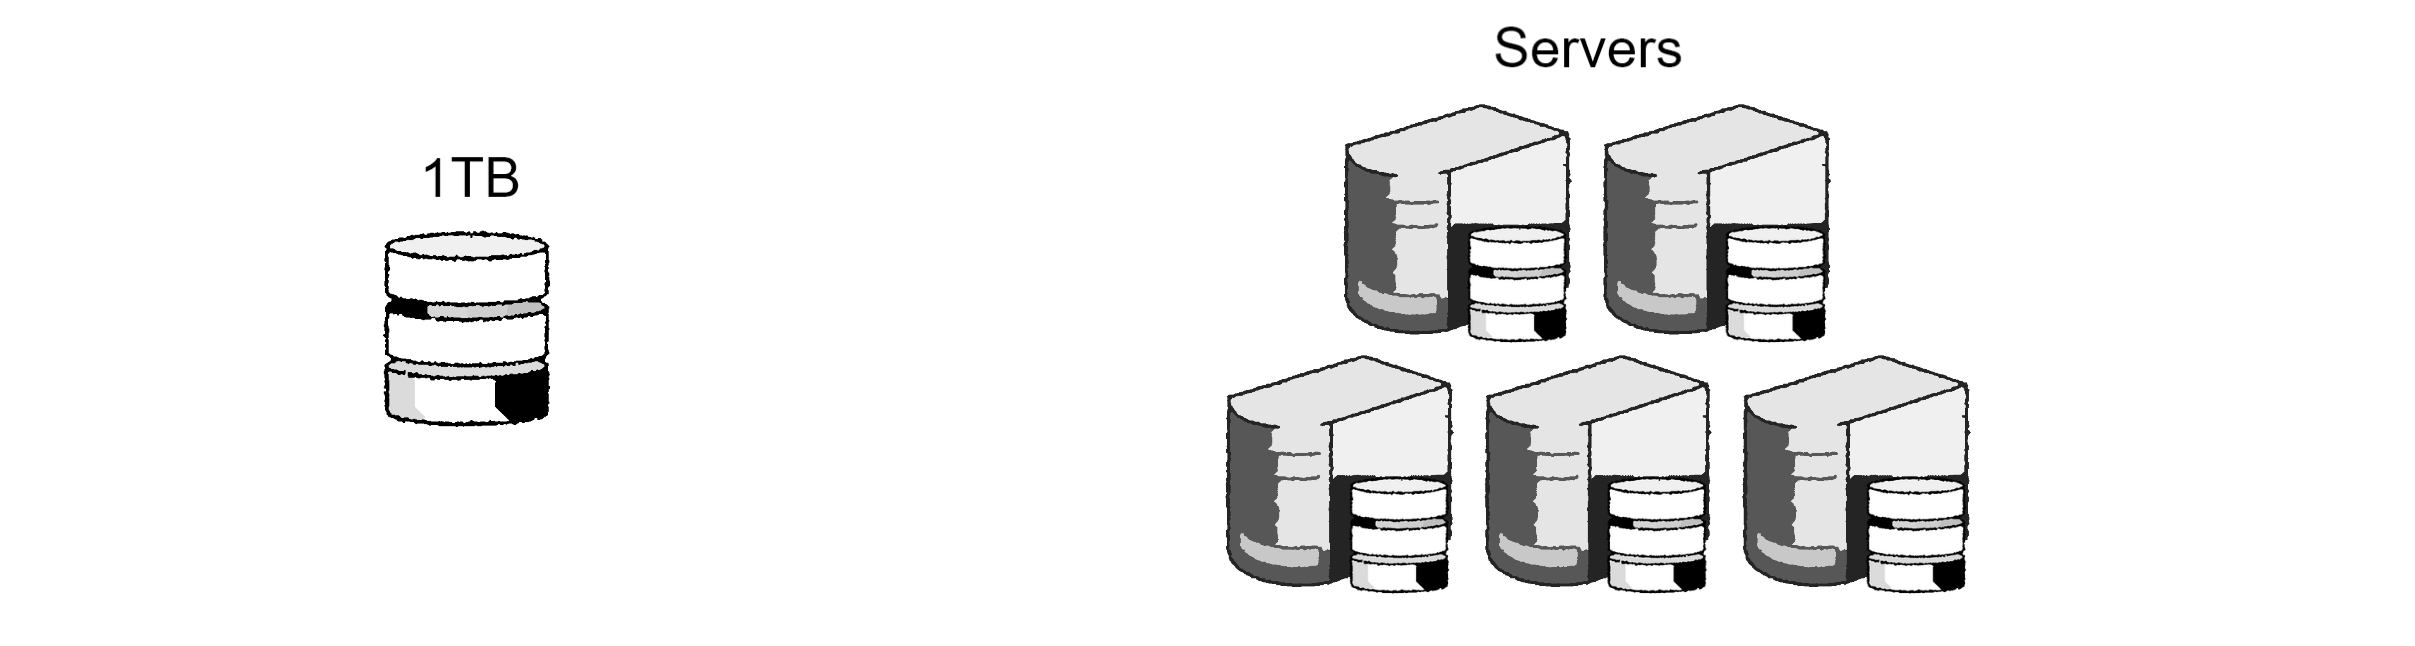
\includegraphics[width=\textwidth]{Sections/shard/server.png}
    \caption{1 TB dataset with 5 servers each with some storage capacity.}
    \label{fig:shard}
\end{figure}

\noindent
Once method is to split up our dataset into 5 partitions, and distribute them across the servers.
\begin{Def}[Sharding]

    \textbf{Sharding} is the process of splitting up a dataset into smaller more manageable pieces called \textbf{shards}. Each shard is stored on a different server, allowing for parallel processing.\\

    \noindent
    In addition, to strengthen fault tolerance, replication could be used to store multiple copies of a single shard on different servers.
\end{Def}

\begin{figure}[h]

    \centering
    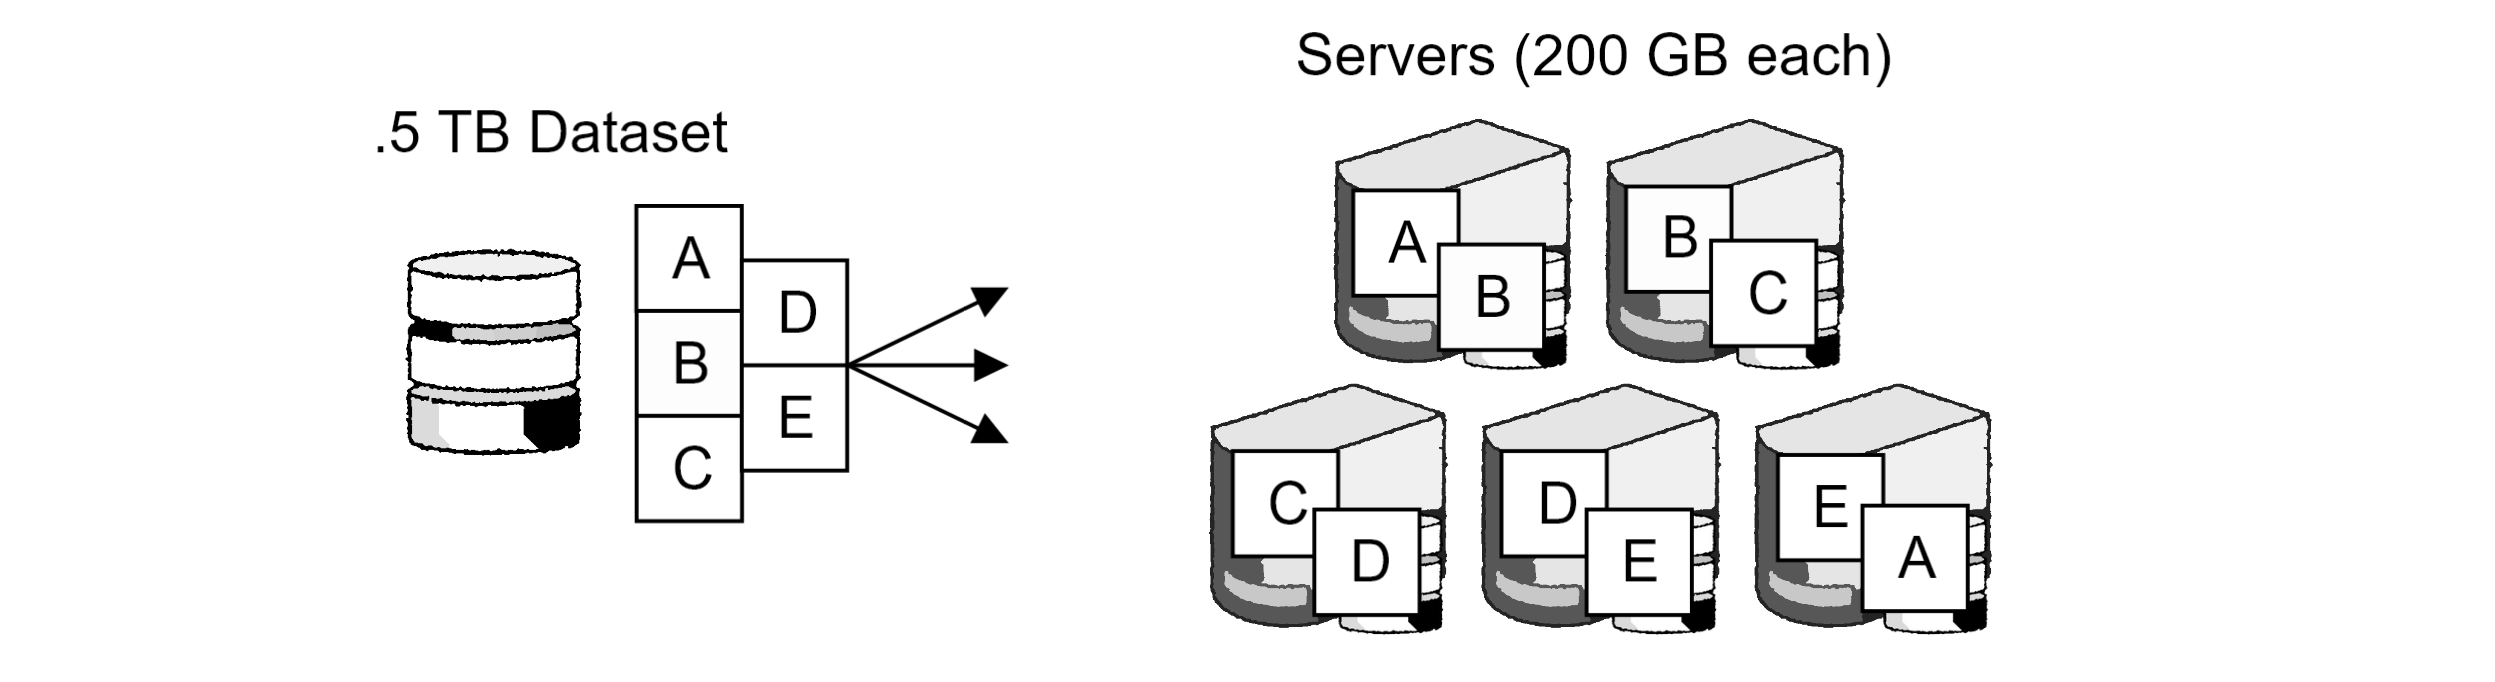
\includegraphics[width=\textwidth]{Sections/shard/shard.png}
    \caption{Sharding a dataset of .5 TB into 5 partitions, each part replicated twice and distributed evenly across 5 servers.}
    \label{fig:shard}
\end{figure}

\noindent
As shown above, shards could be replicated and housed with other shards on the same server.
For instance, this could help in the case that two pieces of data are frequently accessed together.

\newpage 
\noindent
Now we discuss how to assign shards to servers. There are two naive methods:
\begin{itemize}
    \item \textbf{Randomized}: Though statistically balanced, it requires a lookup procedure to find shards.
    \item \textbf{Alphabetical}: Too deterministic, though we skip the lookup procedure.
\end{itemize}

\noindent
Instead we could combine these ideas and use a \textbf{hash function} to map the data to a server:
\begin{Def}[Hash Function]

    A \textbf{hash function} is a function that takes an input (or \textbf{key}) and returns a fixed-size string of bytes. The output is typically a \textbf{digest} that is unique to each unique input.
    Depending on the hash algorithm, the output may be a number or a string of characters, or even produce collisions (two distinct inputs producing the same output).
\end{Def}
\noindent
Ideally the hash function should be:
\begin{itemize}
    \item \textbf{Deterministic}: The same input should always produce the same output.
    \item \textbf{Uniform}: The output should be uniformly distributed across the range of possible outputs.
    \item \textbf{Fast}: The hash function should be fast to compute.
    \item \textbf{Collision Resistant}: It should be hard to find clashing inputs that produce the same output.
\end{itemize}
\noindent
Though this seems fine, it may be costly to deal with migrations:
\begin{figure}[h]
    
        \centering
        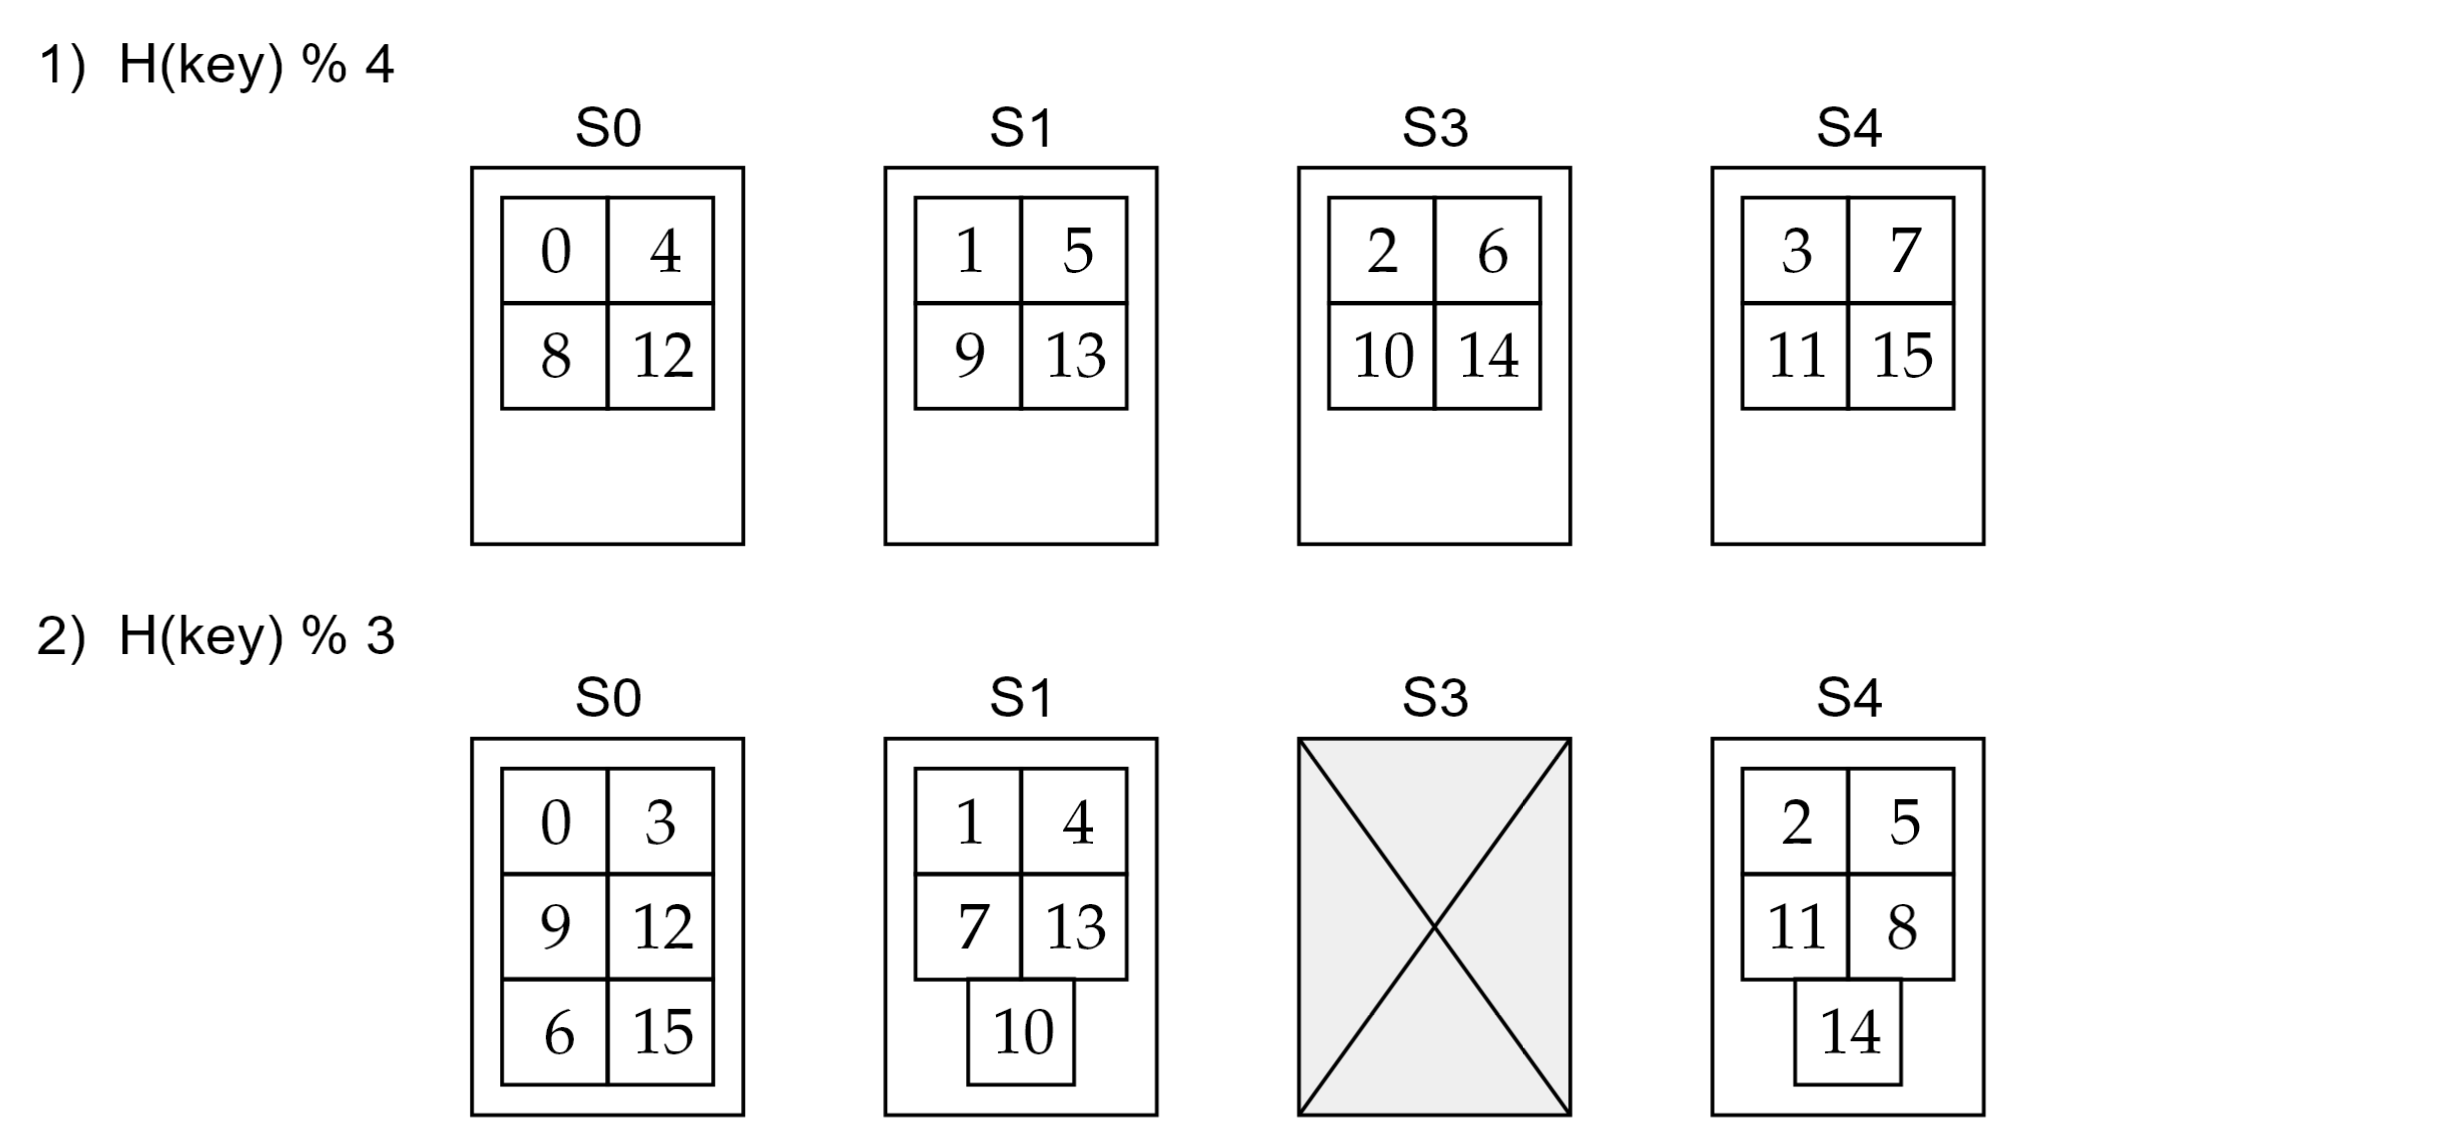
\includegraphics[width=\textwidth]{Sections/shard/mig.png}
        \caption{Given a hash function $H$ and a shard ID $key$, where $H(key)$ returns some server ID -- 1) There are 4 servers utilizing the hash function, using the size of servers
        to modulo overflow. 2) Server 3 goes down, forcing a rehash of the data (unnecessary migration).}
        \label{fig:shard}
\end{figure}

\newpage 
\noindent
To fix this migration problem, we build off the idea of the wrapping modulo overflow behavior, as well as to allow severs to handle multiple hash values:
\begin{Def}[Consistent Hashing (Part 1)]

    \textbf{Consistent Hashing} is a technique used to distribute data across a cluster of servers in a way that minimizes the amount of data that needs to be moved when servers are added or removed.\\

    \noindent
    Here the hash function $H$ maps keys to an $m$-bit value, which provides a hash-space of $2^m$. I.e.,
    we have $2^m$ possible hash values ($\{0,1,\ldots,2^m-1\}$), which forms a ring, allowing us to wrap around the hash space.

    Then servers $S_i$ often called \textbf{virtual nodes} or \textbf{virtual replicas}, are evenly assigned a portion of the ring to cover. Any hash that falls within this range is assigned to the server.
    If a server $S_i$ goes down, its range is passed to the next server $S_{i+1}$ (without having to rehash the data).
\end{Def}

\begin{figure}[h]
        
            \centering
            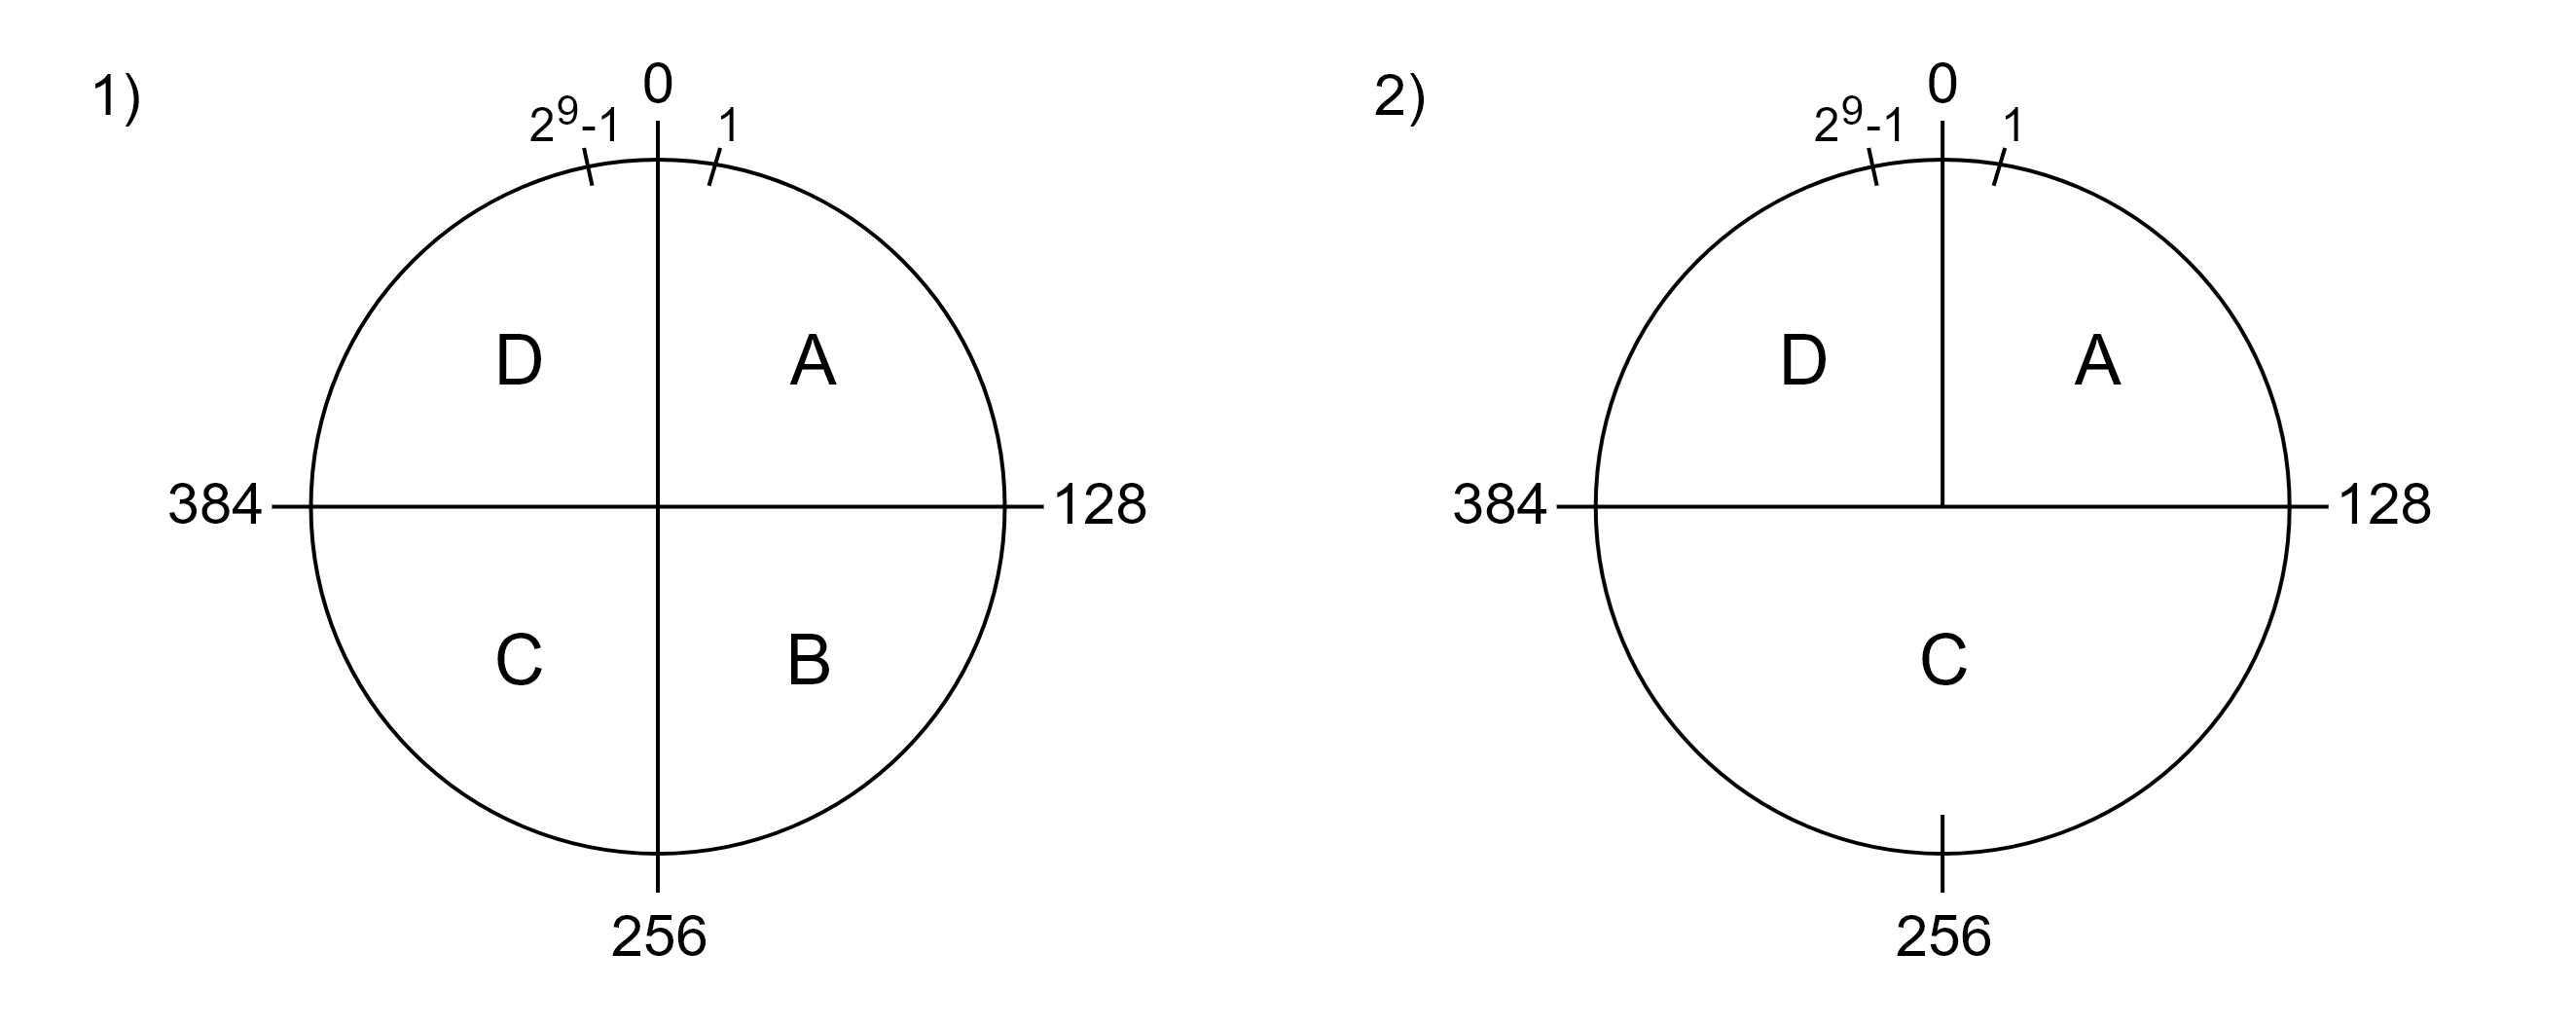
\includegraphics[width=\textwidth]{Sections/shard/ring.png}
            \caption{A consistent hashing ring of 9-bit values (512 possible values). The ring includes 4 servers $A,B,C,D$. 2) Server $B$ goes down, transferring its range to $C$.}
            \label{fig:ring}
\end{figure}

\noindent 
In Figure (\ref{fig:ring}) in part 2, the data is \textbf{no longer evenly distributed} across servers after a lost server. Likewise, the 
same problem occurs when adding a server. We mitigate this via the following:

\begin{Def}[Consistent Hashing (Part 2)]
    \noindent
    To achieve an even distribution of virtual nodes, we in essence take server $S_i$'s range and split it into $k$ slices, distributing them evenly across the ring.\\

    \noindent
    In particular, given $n$ servers, and a ring of size $2^m$, we create $k$ virtual nodes to each server, requiring $k$ different hash functions for server assignment.
    Typically, $k\approx \log_2(2^m)=m$. \hfill \cite{RoughgardenValiant2024CS168L1}
\end{Def}

\newpage 

\noindent
Below we illustrate how just a basic implementation of this improves our load balancing:
\begin{figure}[h]
        
            \centering
            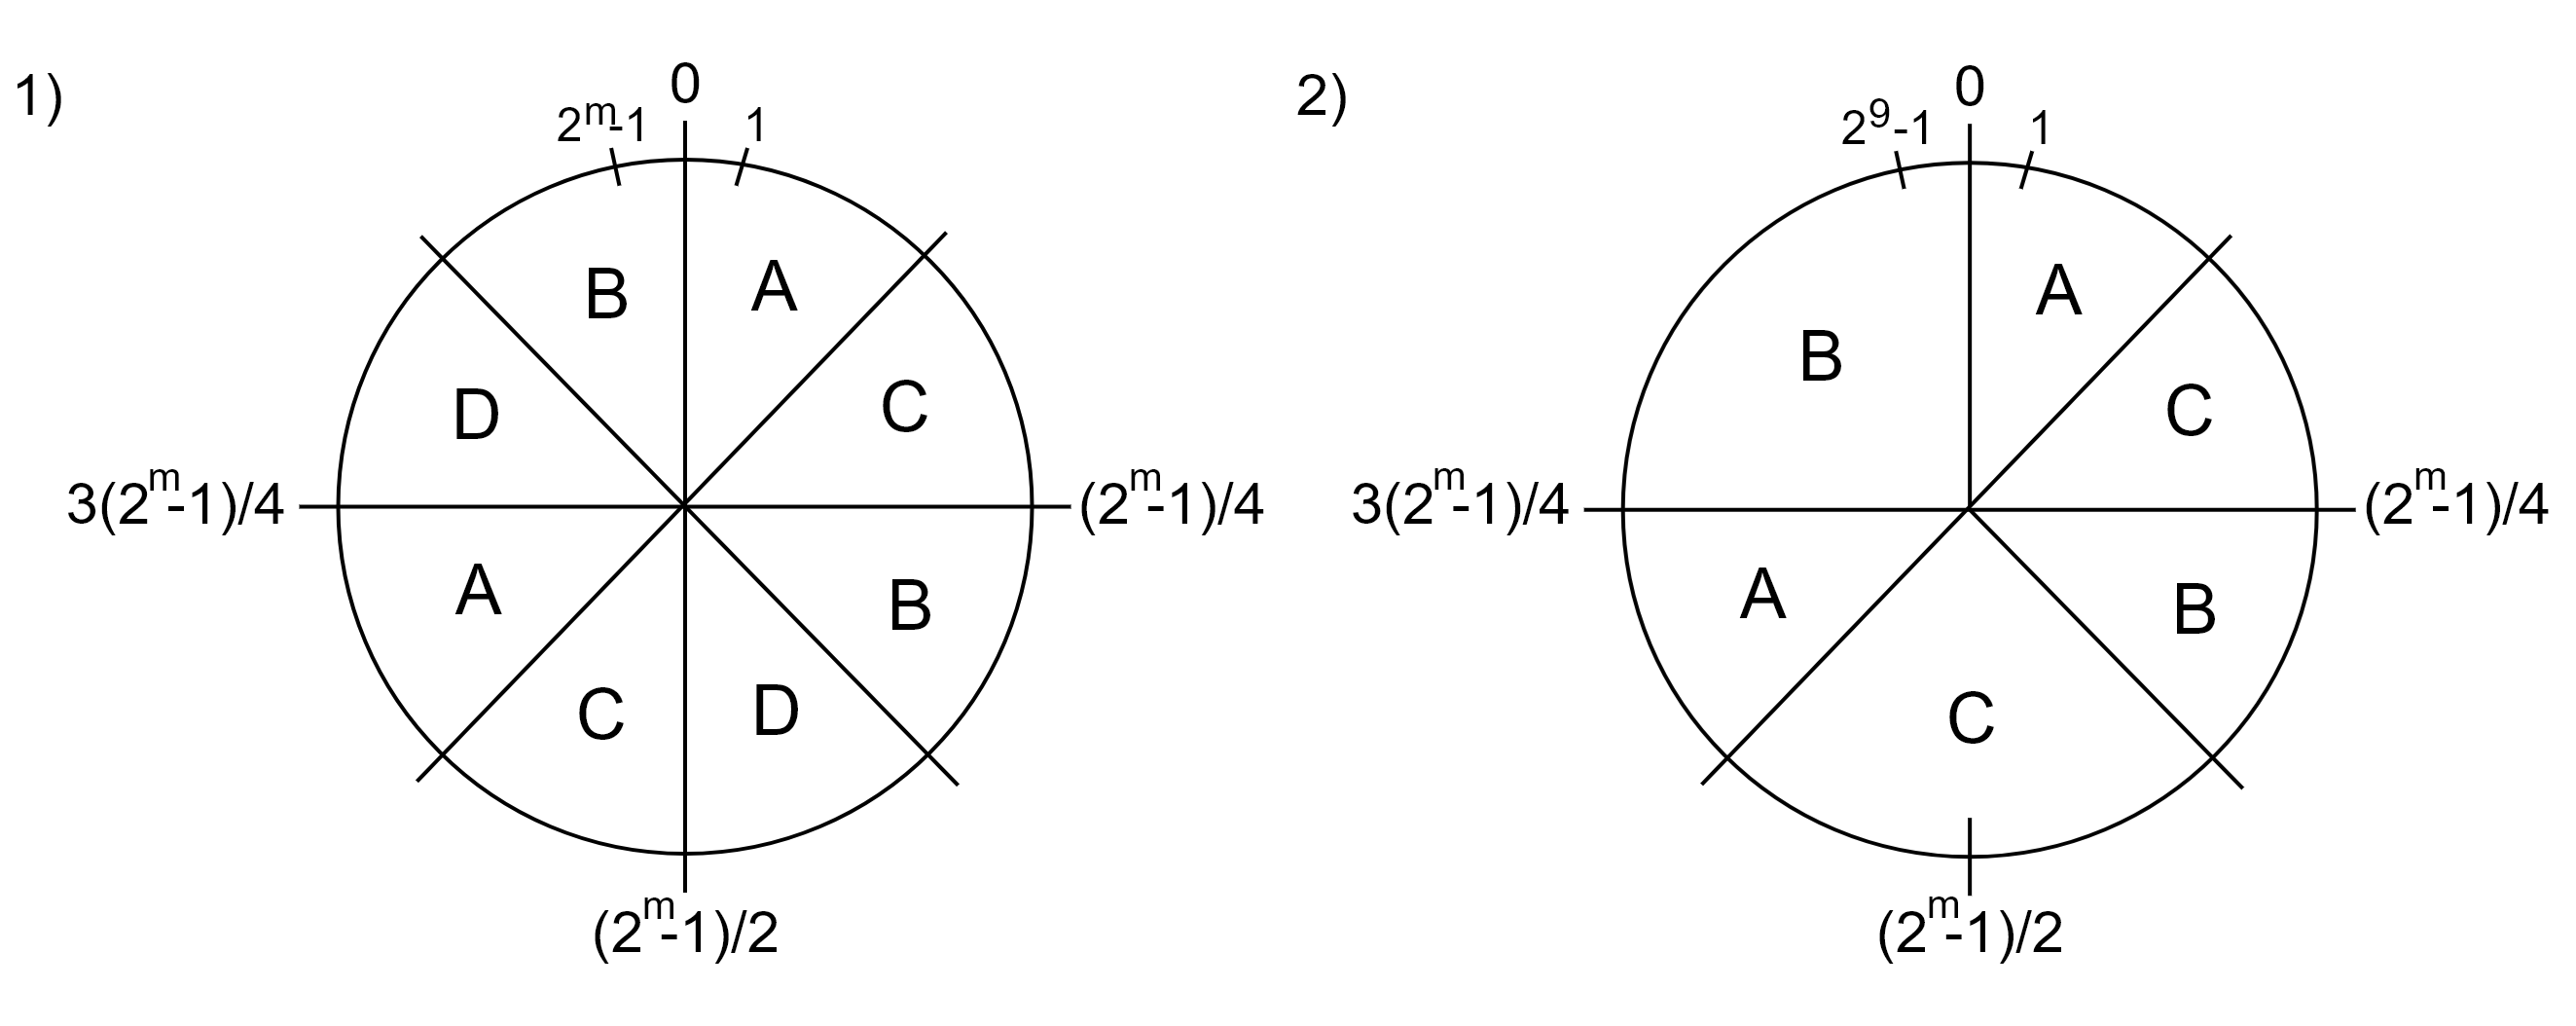
\includegraphics[width=\textwidth]{Sections/shard/ring_2.png}
            \caption{A consistent hashing ring of m-bit values, where we choose $k=2$ splits for $n=4$ servers across the ring.
            1) All 4 servers and their replicated virtual nodes in even distribution. 2) Server $D$ goes down, transferring its range to $B$ and $C$.}
            \label{fig:ring_2}
\end{figure}

\noindent
In the above figure, choosing just $k=2$ makes a huge difference as opposed to our previous solution in Figure (\ref{fig:ring_2}).